\begin{figure}[t!]
  \centering
  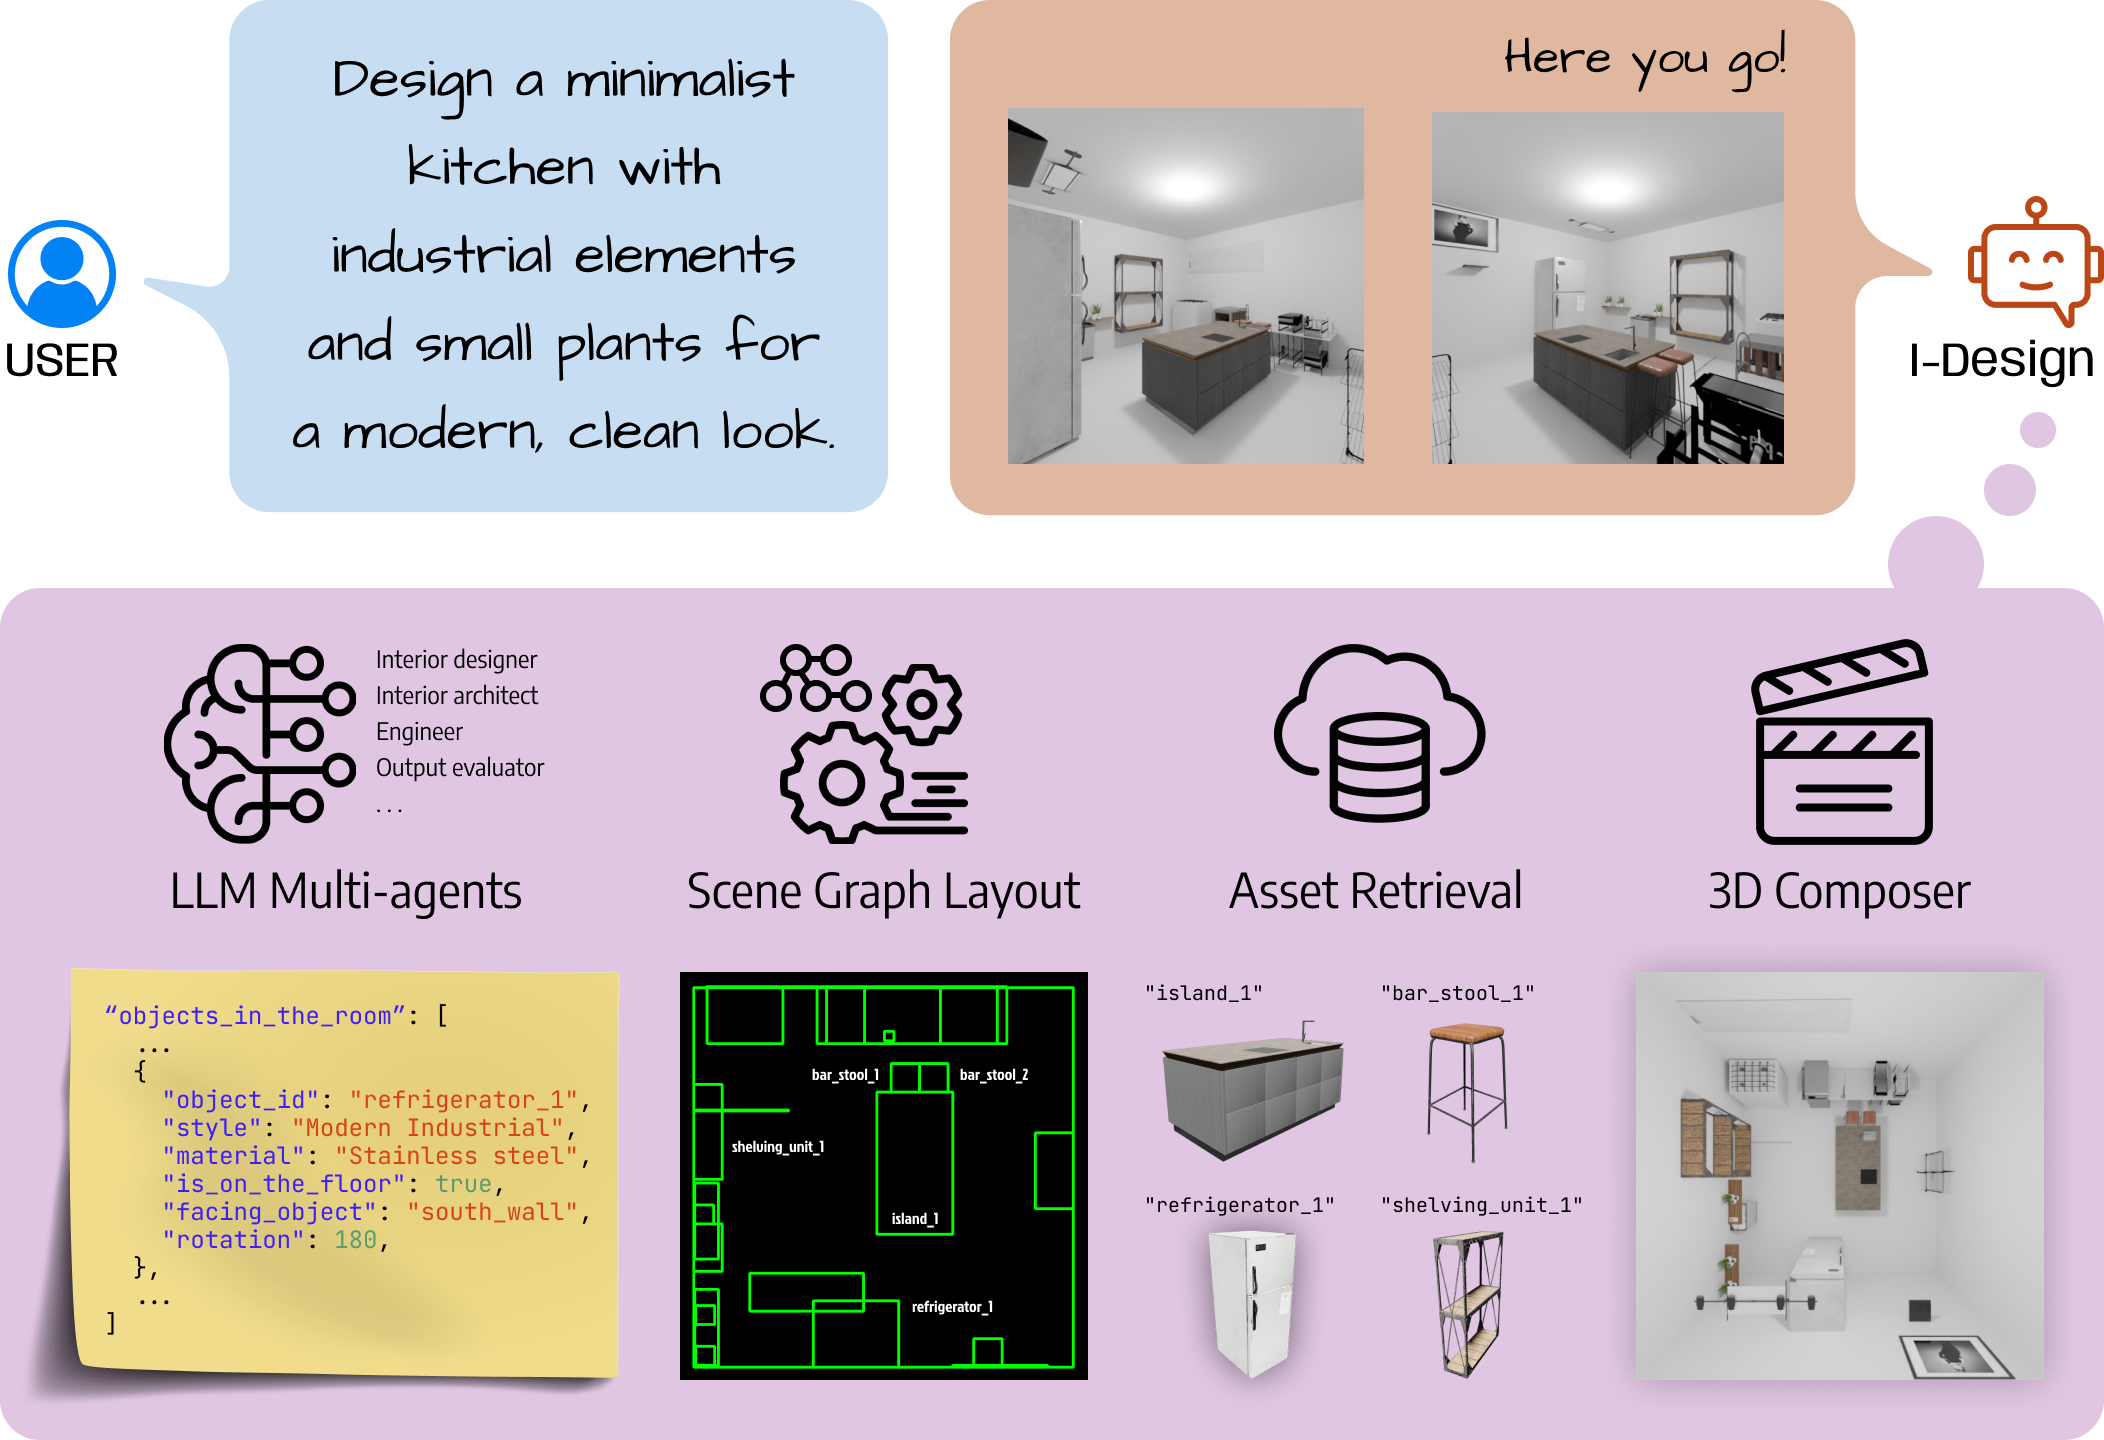
\includegraphics[width=1.0\textwidth]{images/overview.png}
  \caption{
    \textbf{Overview of \methodname.}
    Starting from the user specification of design preferences in plain text, we query LLM agents to come up with room items, their properties, and their relative relationships in the form of a scene graph. We solve for absolute object placement in the scene graph using the proposed backtracking algorithm (Scene Graph Layout), retrieve 3D assets according to the functional and stylistic specifications, and compose the final result in 3D.
  }
  \label{fig:overview}
\end{figure}
